% Zusammenfassung und Ausblick
%

\chapter{Discussion}

\section{Circuit properties}


The generated full mouse brain circuit contains around 74 million neurons and 660 billion synapses.
The simulation uses 12 parameters from the neuron file.
It contains further parameters which are used for the connection generation and the visualization,
like coordinates. In total the neuron file is around 9 GB.
The synapse file only contains needed parameters for the simulation.
There are five synapse parameter per connection. This results in 15 TB of data
for the long range connectivity and 600 GB for the short range connectivity.
All in all, the generated circuit contains around 16 TB of data and it is split in three HDF5
files (neuron file, long range synapses file and short range synapses file).

The interpolation, which are applied to the long range connection generation, introduces errors.
For illustration Figure \ref{interpolationdistance} shows the locality of missing voxels in one slice.
The quality of the interpolation can be estimated from the distance (color scale in Figure).
The distance corresponds to the distance from the nearest neighbour search algorithm.
It highlights problematic regions.
\begin{figure}[ht!]
\centering
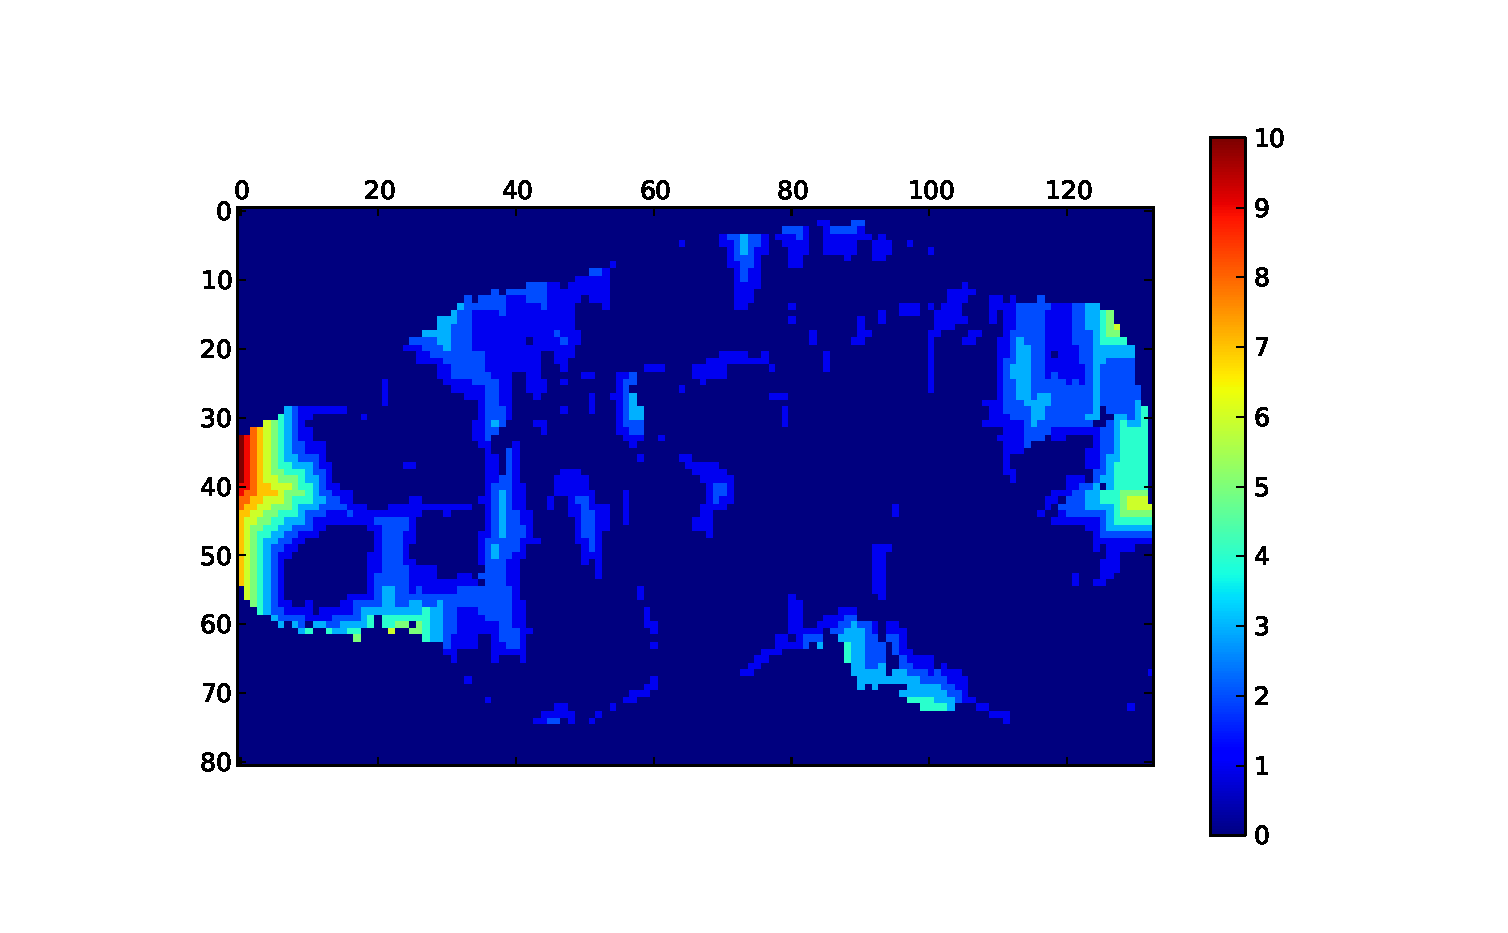
\includegraphics[scale=0.5]{pictures/distance_x_y_70.eps}
\caption{Plotted values from the nearest neighbor algorithm. You can see the distance to the next injected voxel.}
\label{interpolationdistance}
\end{figure}
But the interpolations enable generation of a full mouse brain model from incomplete experimental data.
This full mouse brain model can be loaded inside of NEST with the implemented modules.
If there are more experiments available they can be included into
the circuit generation easily.

\begin{table}[ht!]
\begin{centering}
    \begin{tabular}{ | l | l | r | r | r |}
    \hline
    Identifier & ratio & neurons & synapses & total size \\ \hline \hline
    threehundredths & $0.3\%$ & $~2.5*10^5$ & $~2.2*10^9$ & $~26$ GB \\ \hline
    quater & $25\%$ & $~1.9*10^7$ & $~1.6*10^{11}$ & $~4$ TB \\ \hline
    full & $100\%$ & $~7.5*10^7$ & $~7.2*10^{11}$ & $~16$ TB \\ \hline
    \end{tabular}
    \caption{The circuits \emph{3hundredths}, \emph{1quater} and \emph{full} were created for testing and debugging on different scales.
All circuits were generated with identical parameters, only the input neuron file varies.}
\end{centering}
    \end{table}


\label{table:circuits}

Three different circuits (see Table \ref{table:circuits}) are generated: The full mouse brain circuit,
a smaller circuit that contains 25 percent of the full mouse brain circuit and
$\frac{1}{300}$ of the full circuit. The percentage is related to the number of neurons inside
the circuit. The connections are generated based on the neurons. In principle the
number of connections should be of the same proportion.

\section{Data format usability}
The HDF5 data format for neuron parameters is used as given from the Neurorobotics team of the Blue Brain Project.
Because of its small size (9 GB) in comparison to the synapse dataset (15 TB) the performance improvement by changing
to a transposed data format can be neglected. Thus the advantage of having different datasets and being able
to add new datasets can be kept. It also implies that the generation script does not have to be converted or no 
conversion scripts are needed.


\section{Long range connections generation}
Moving the best injection per voxel search outside the main iteration
avoids unnecessary calculations and reduces the complexity of the main iteration.
In the sequential algorithm parts of the connections are regenerated in each iteration.
This is avoided by looking for the best injection per voxel beforehand.


Optimization of the linear acceptance rejection function (see \ref{par:linearacceptancerejection})
reduces the complexity of picking from number of neurons in projection to number of voxels in projection.
For the full circuit this corresponds to a reduction of the order of 2.
Using all core inside the function gives a further speed up.
Each thread has to pick $~\frac{10,000}{N_{threads}}$ voxels instead of
$10,000$.

The program execution takes around around 15h on the Blue Brain IV using 2048 processes for the full circuit.
Each processes uses all threads. Optimized collective writing operations could 
lower the needed execution time.
But is not feasible, because the generation script will be executed only a few times
and the computational resources are given.



\section{Short range connections generation}
The sequential algorithm could be ported directly to a parallel implementation without changing it.
Using a Master-Slave approach also reduced the complexity of the distribution of independent iterations.
The critical part of the implementation is the IO, because the number of created synapses is not known in the beginning.
Therefore the file size can not calculated beforehand, which is mandatory for an efficient writing to HDF5 files. 
By using a buffer or temporary files this problem can be avoided.
Because of the given resources (Blue Brain IV) and the high parallel efficiency (see later section)
writing all synapses to a buffer is feasible (already for a small number of nodes the created connections fit in memory).
The buffer implementation, which behaves like a queue, is efficient in terms of writing to disk and writing to file
if the queue chunks are large enough. Using larger chunks leads to 
a higher utilization of the theoretical bandwidth. Additionally, it leads to less write independent,
write operations, which reduces the waiting time in serialization mechanisms.

The program execution takes around around 0.5h on the Blue Brain IV using 256 processes for the full circuit.
Two tasks per process are launched. Optimizing the load balance could lead a better performance.
But is not feasible, because the generation script will be executed only a few times
and the computational resources are given.

\section{Import circuit}
Loading the mouse brain model inside of NEST is the main goal of the thesis.
Therefore NEST is extended with two import modules, which allow to import the
generated mouse brain model. To show that the implemented algorithms are feasible 
the circuit properties, which effect the load balance, are analysed.
Afterwards the performance characteristics of the implemented algorithm are shown.

The IO performance of the implementation affects mainly the usability.
Runs on different scales should give detailed information about the reached bandwidth.
The bandwidth is calculated by:
\begin{equation}
  bandwidth = bytes~per~synapse * \frac{number~of~synapses}{\Delta t} [\frac{Bytes}{s}]
\end{equation}
In priory the \emph{connect} task was detected as the bottleneck of the algorithm on scales up to 2 racks on IBM Blue Gene Q.
A thread-parallelization of the \emph{connect} task achieved a speed-up.

Two weak scaling and one strong scaling scenarios were tested.
The properties are listed in table \ref{schumann:tbl:runs}.
\begin{table}[h!]
  \caption{Properties of scaling runs}
\begin{center}
\begin{tabular}{|r|l|p{1.5cm}|p{1.4cm}|p{1.4cm}|p{3cm}|}
\hline
id & scaling & importing & mpi ranks per node & threads per mpi rank & bg\_sizes \\
\hline\hline
1.    &  strong  & $1.9$ $TB$             & 1 & 16 & 1024, 2048, 4096, 8192, 16384, 28672 \\
2.    &  weak  & $900$ $\frac{MB}{node}$      & 1 & 16 & 1024, 2048, 4096, 8192, 28672 \\
3.    &  weak  & $220$ $\frac{MB}{node}$     & 1 & 16 & 1024, 2048, 4096, 8192, 16384, 28672 \\
\hline
\end{tabular}
\end{center}
\label{schumann:tbl:runs}
\end{table}
\begin{figure}[h!]
\begin{center}
 \includegraphics[width=0.8\textwidth]{pgfplots/bandwidth.pdf}
\end{center}
\caption{Bandwidth comparison of different scaling runs (see table \ref{schumann:tbl:runs}).
The plotted values are taken from Table \ref{schumann:tbl:scalruns}.
The \emph{theoretical} line shows the approximate maximum bandwidth of the system.}
\label{schumann:fig:bandwidth}
\end{figure}
Figure \ref{schumann:fig:bandwidth} plots the bandwidth measured for the runs over number of nodes.
The resulted bandwidths tackles around five percentage of the theoretical bandwidths.
All runs give similar results.
A more detailed look on the task scale should give more insights.
An instrumented version of the algorithm with scorep gives us wall-clock timings of each task per node.
We are interested in bottlenecks.
Therefore we look at the proportions of the tasks (see Figure \ref{schumann:fig:taskratios}).
\begin{figure}[h!]
\begin{center}
 \includegraphics[width=0.5\textwidth]{pgfplots/taskratios.pdf}
\end{center}
\caption{Measured task durations percentages of the total duration on different scales.
 The displayed percentages are the means of percentages for all nodes.
 The values are extracted from the 1. scaling run (see table \ref{schumann:tbl:runs}).
 }
\label{schumann:fig:taskratios}
\end{figure}
Apparently, \emph{load} and \emph{alltoall} effect mainly the run time of our module.
\emph{load} performs io. It uses the HDF5 library to load synapses from disk to the internal data structure.
\emph{alltoall} exchanges synapses between the ranks. Both tasks contain collective MPI calls.
A detailed look at the call stack of the used H5Read function shows that the called MPI read operation is non-collective.
Using the HDF5 property list interface we identify that the internal data structure of the import module prevents HDF5 from using collective read operations.
A collective read operation could result in better read performance.
Therefore a comparison of collective versus independent read operations should show possible benefits.
Because of the limited time we focus on the comparison of a reduced algorithm,
which allows an easy change of the used data structure.
We can provide two test implementations with and without adapted data structure.
\begin{figure}[h!]
\begin{center}
 \includegraphics[width=0.8\textwidth]{pgfplots/bandwidth_stats.pdf}
\end{center}
\caption{Comparison of achieved bandwidth from collective versus independent read operations.
 Values from table \ref{schumann:tbl:indevscol} are used. Theoretical line shows the limits by the
 JUQUEEN system.}
\end{figure}
The new algorithm reduces the iterations to the \emph{load} part with a following MPI barrier.
The MPI barrier should simulate any \emph{collective} read operations inside of the \emph{alltoall} task.
\begin{figure}[h!]
\begin{center}
 \includegraphics[width=0.5\textwidth]{pgfplots/indiVScollec.pdf}
\end{center}
\caption{Comparison of collective versus independent read operations executed on 16 racks.
 Values are extracted from the scorep measurements from the runs listed in table \ref{schumann:fig:indiVScollec}.}
 \label{schumann:fig:indiVScollec}
\end{figure}

Figure \ref{schumann:fig:indiVScollec} illustrates the benefit of collective versus independent read operations
on the JUQUEEN system for 16 racks.

Even tough the mean time of the read operations is similar, the serializations of the read calls effects the
imbalance and therefore the idle times at the next collective operations. 

Therefore a change in the data structure should bring great benefit for our implementation.
We are confident that the optimization will result in better usage of the available bandwidth.
Even tough large scale data-driven simulation are already possible with the developed import module for NEST,
further optimization on the algorithm can increase the bandwidth and therefore lower the needed time.
Taking into account that large scale data-driven simulations are getting more of interest as more 
data is available, we are going to spend more effort in the optimization of the import module.


\begin{table}[h!]
  \caption{Scaling runs of the import module using independent read calls on JUQUEEN. \emph{1.times}, \emph{2.times} and
  \emph{3.times} corresponds to the times of the 1., 2. and 3. scaling runs (see table \ref{schumann:tbl:runs}).}
\begin{center}
\begin{tabular}{|r|r|r|r|r|r|}
\hline
bg\_size& rpn & MPI ranks & 1. time[s] & 2. time[s] & 3. time[s] \\
\hline\hline
1024    &  1  & 1024      & 1222 & 523 & 123 \\
2048    &  2  & 2048      & 642  & 593 & 118 \\
4096    &  2  & 4096      & 363  & 661 & 139 \\
8192    &  4  & 8192     & 325  & 827 & 245 \\
16384   &  8  & 16384    & 208  & -   & 364 \\
28672   & 16  & 28672    & 168  & 1401& 497\\
\hline
\end{tabular}
\end{center}
\label{schumann:tbl:scalruns}
\end{table}

\begin{table}[h!]
  \caption{Scaling runs of test implementation to compare collective versus independent read calls on JUQUEEN. \emph{bytes~per~synapse} is $24$ for all runs.}
\begin{center}
\begin{tabular}{|r|r|r|r|r|r|}
\hline
bg\_size& rpn & MPI ranks & mpiio & synapses in buffer & time[s] \\
\hline\hline
2048    &  2  & 2048      & independent  &  9395240960 & 36.7041712582\\
4096    &  4  & 4096      & independent  & 9395240960  & 21.6904791038\\
16384   &  16  & 16384      &  independent & 300647710720  & 406.885908909\\
512     &  0.5  & 512      & collective  & 9395240960  & 70.67277588\\
2048    &  2  & 2048      & collective  & 9395240960  & 29.0894202424\\
4096    &  4  & 4096      & collective  & 9395240960  & 12.5637469038\\
8192    &  8  & 8192      & collective  &  9395240960 & 7.9934176194\\
16384   &  16  & 16384      &  collective & 300647710720  & 191.27968665\\
\hline
\end{tabular}
\end{center}
\label{schumann:tbl:indevscol}
\end{table}

\subsection{Load balance}
The neurons are distributed equably on all processes based on equation \ref{eq:processfromid}.
But the number of incoming synapses varies between the neurons.
Therefore a memory imbalance could occur between the processes.
To analyse the imbalance, an analysing script iterates over the \emph{syn} dataset and counts
the number of incoming synapses per neuron. Normalized results are plotted in box-plot diagrams 
in Figure \ref{fullcircuitdist}.
It shows an increasing imbalance of synapses per process with increasing number of processes.
\begin{figure}[ht!]
\centering
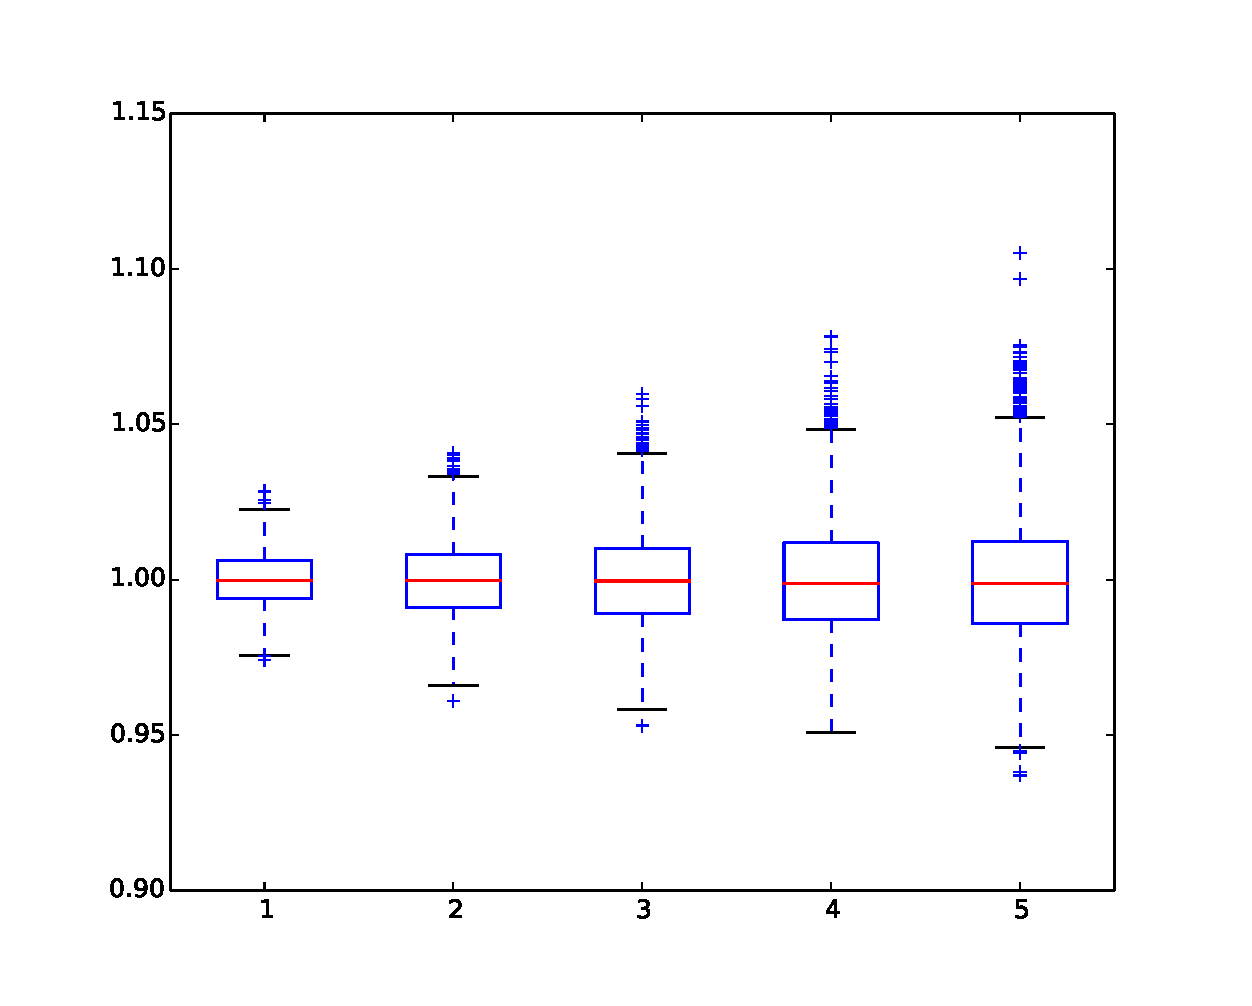
\includegraphics[scale=0.4]{pictures/full_circuit_rack_distribution.eps}
\caption{Estimated synapse imbalance of neuron distribution on processes.
It shows the distributions of relative sums (sum of number of synapses per process divided by mean of sums) of synapses per process (y-scale) on different scales (x-axis). Relative sums means absolute sums devided by the mean sum per process. }
\label{fullcircuitdist}
\end{figure}

\subsection{Speed-up}
Four parts of the synapse loading algorithm are instrumented to get wall clock timings.
\emph{Read}, \emph{Sort}, \emph{Alltoall} and \emph{Connect} are considered to be the mots time
consuming parts of the algorithm. The parts relate to figure \ref{fig:shortrangeparallel}.
\emph{Def. Node} is negligible (It takes less than 1 percent computation time of an iteration and scales constant with the number of nodes.).
The following figures \ref{fig:implV03} give an overview of the measured wall-clock timings.
The timings are shown per node and iteration number. They give an idea how the timings are distributed.
The performance of the different parts can be compared and bottlenecks can be found.
Runtime measurements of the import module are performed at different scales.
Therefore IBM Blue Gene /Q systems in Lugano (Blue Brain IV) and Juelich (JUQUEEN) are used.
%\begin{figure}[ht!]
%     \begin{center}
%        \subfigure[Load hdf5 files]{%
%            \label{fig:first}
%            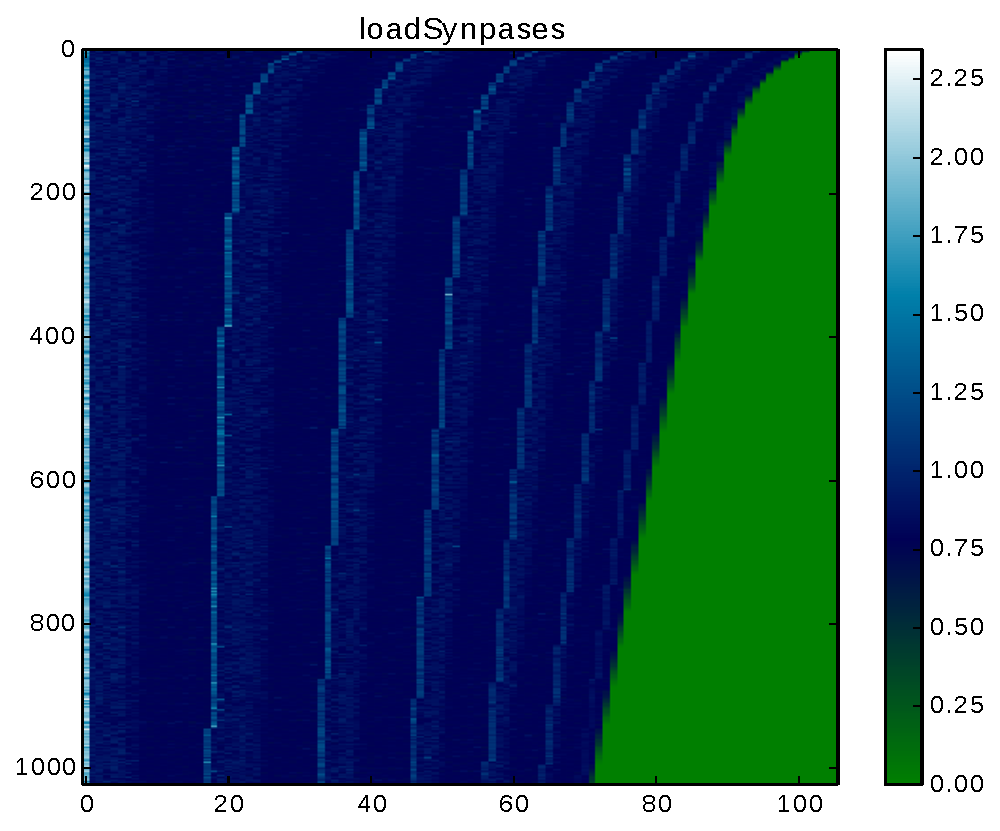
\includegraphics[width=0.45\textwidth]{pictures/V03_loadSynapses.eps}
%        }
%        \subfigure[Sort connection information data by target node]{%
%           \label{fig:second}
%           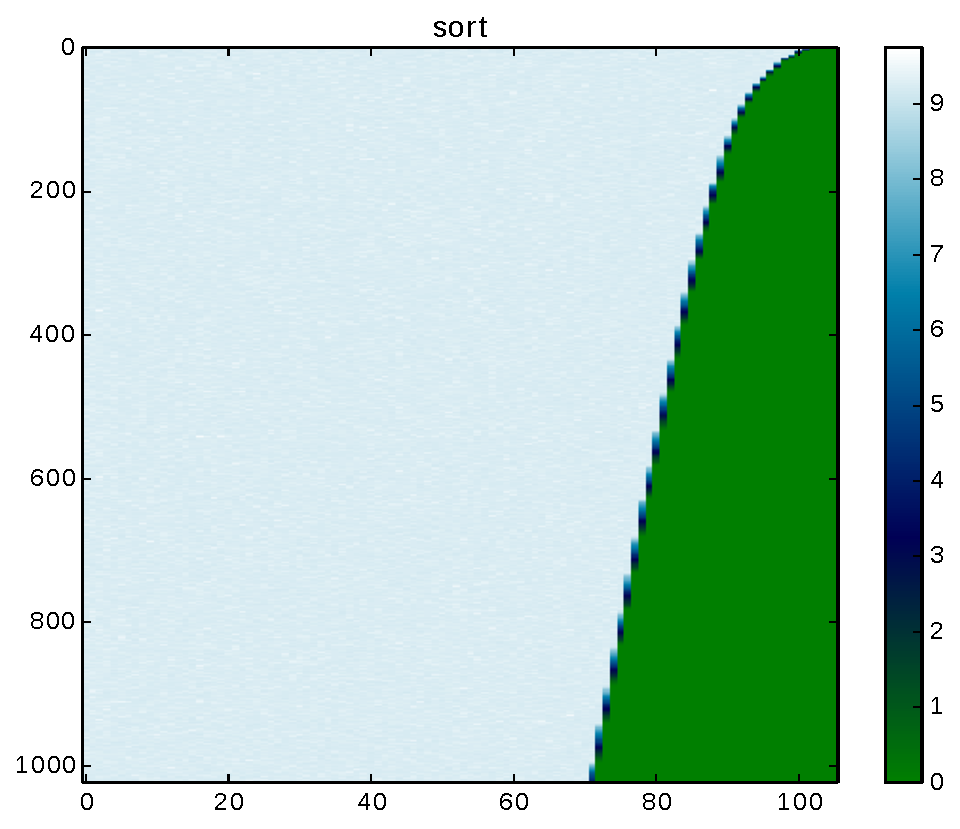
\includegraphics[width=0.45\textwidth]{pictures/V03_sort.eps}
%        }\\ %  ------- End of the first row ----------------------%
%        \subfigure[Send data to all target nodes using AlltoAllv]{%
%            \label{fig:third}
%            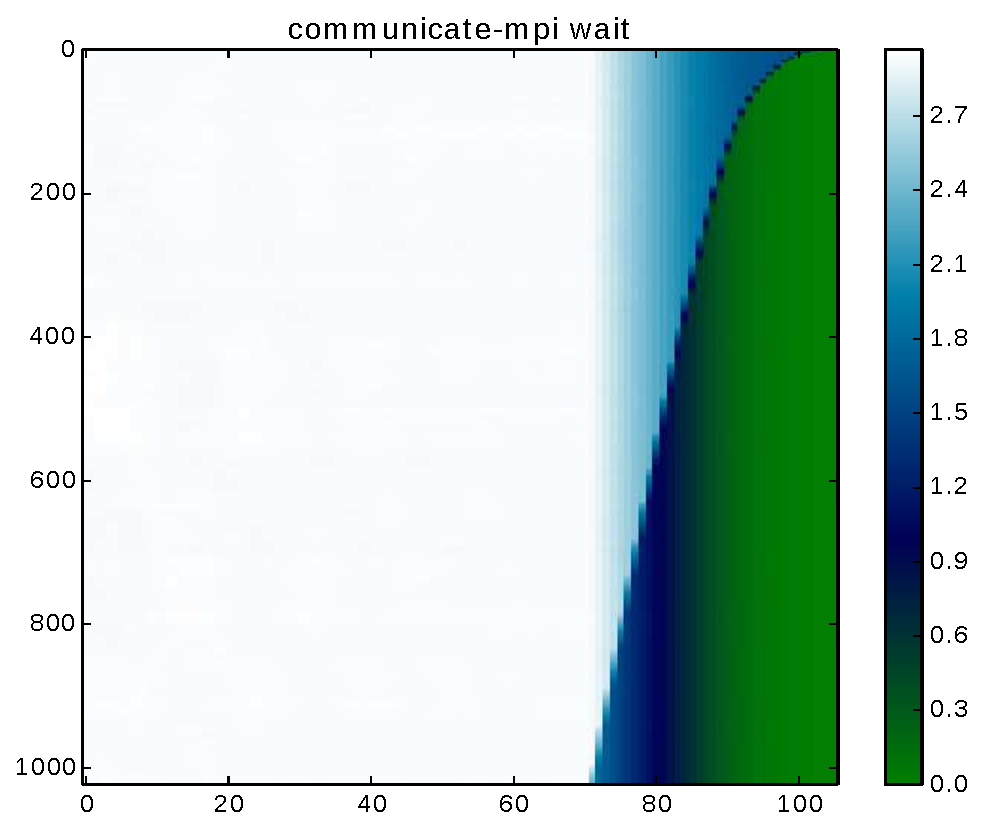
\includegraphics[width=0.45\textwidth]{pictures/V03_communicate.eps}
%        }
%        \subfigure[Connect function which calculated delay and calls NEST connect]{%
%            \label{fig:fourth}
%            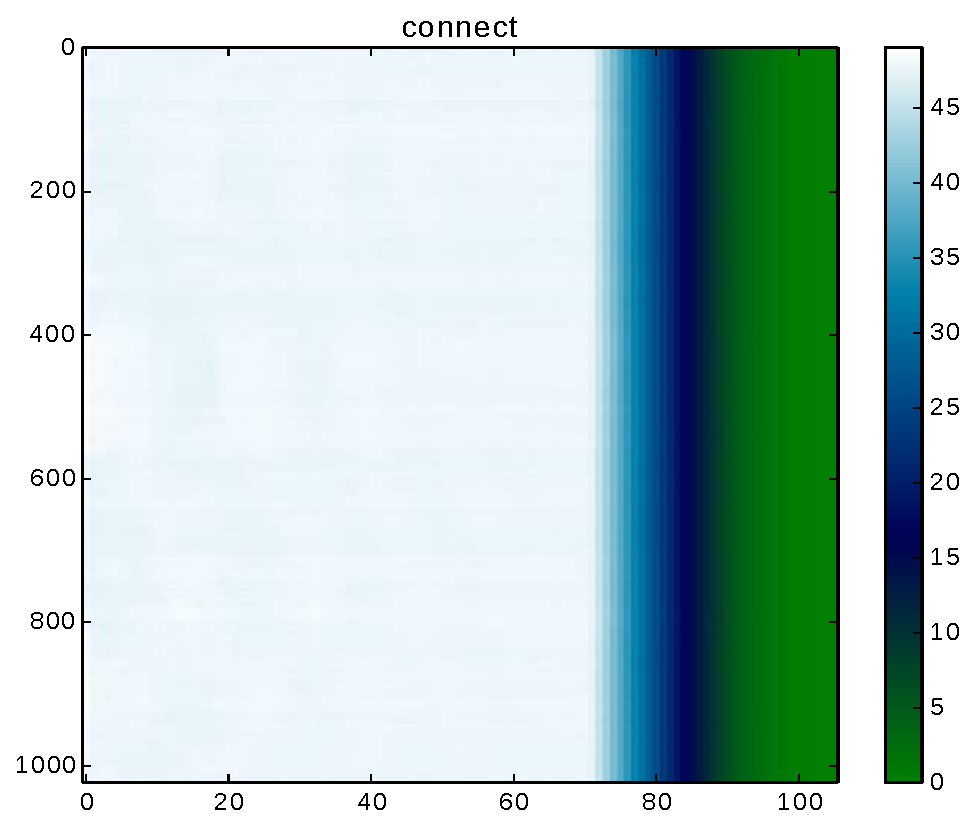
\includegraphics[width=0.45\textwidth]{pictures/V03_connect.eps}
%        }
%    \end{center}
%    \caption{%
%        The the plots show the the execution time for node per iteration.
%        The y-axes corresponds to the node id and the x-axes corresponds to the iteration number.
%        The color scale is in seconds.
%        In each iteration loadSynapses loads max $1e6$ synapses from hdf5 file.
%     }%
%   \label{fig:implV03}
%\end{figure}
One can see that \emph{Read} and \emph{Connect} are the critical parts.
For the interpretations of the plots one has to take into account that different parts of the algorithm
(\emph{Read} and \emph{Alltoall}) contain mpi collective operations and contain therefor mpi waits.
Thus the wall-clock timings do not satisfy the pure step duration but also the imbalance from previous steps.
To analyse the impact, an experiment is performed which extends the implementation with \emph{MPI\_Barriers}
between the algorithm steps.
\newpage
\subsection{Read step}
The efficiency of the \emph{Read} step is bounded by the IO bandwidth of the system.
Blue Brain IV has a theoretical bandwidth of $8$ GB/s per rack.

The amount of data read in \emph{Read} step depends on the number of synapse parameters $N_{params}$,
the number of read synapses per iteration $N_{blocksize}$ and the number of processes $N_{processes}$.
This results in a measured bandwidth of:
\begin{equation}
b = sizeof(float) * N_{params} * \frac{N_{blocksize} * N_{processes}}{\Delta T}
\end{equation}
\subsection{Connect step}

Thread parallelization of the connect step allows to store the synapses efficiently in the NEST data structure.
The pure connect functionality of NEST is thread-safe. But creating and destroying SLI data objects is not and can result
in data-races. To overcome this limitation the creation and destroying of the objects is serialized.
Before iterating over all synapses one SLI object is created and destroyed afterwards for each thread.
A single connect function call of the NEST api expects the synapse parameters stored in a SLI object.
In each iteration the current parameters are assigned to the values inside the already created SLI object.
This SLI object is passed to the function call.
Thus a small overhead for the creation and destroying of the object are perceived.
\begin{figure}[ht!]
\centering
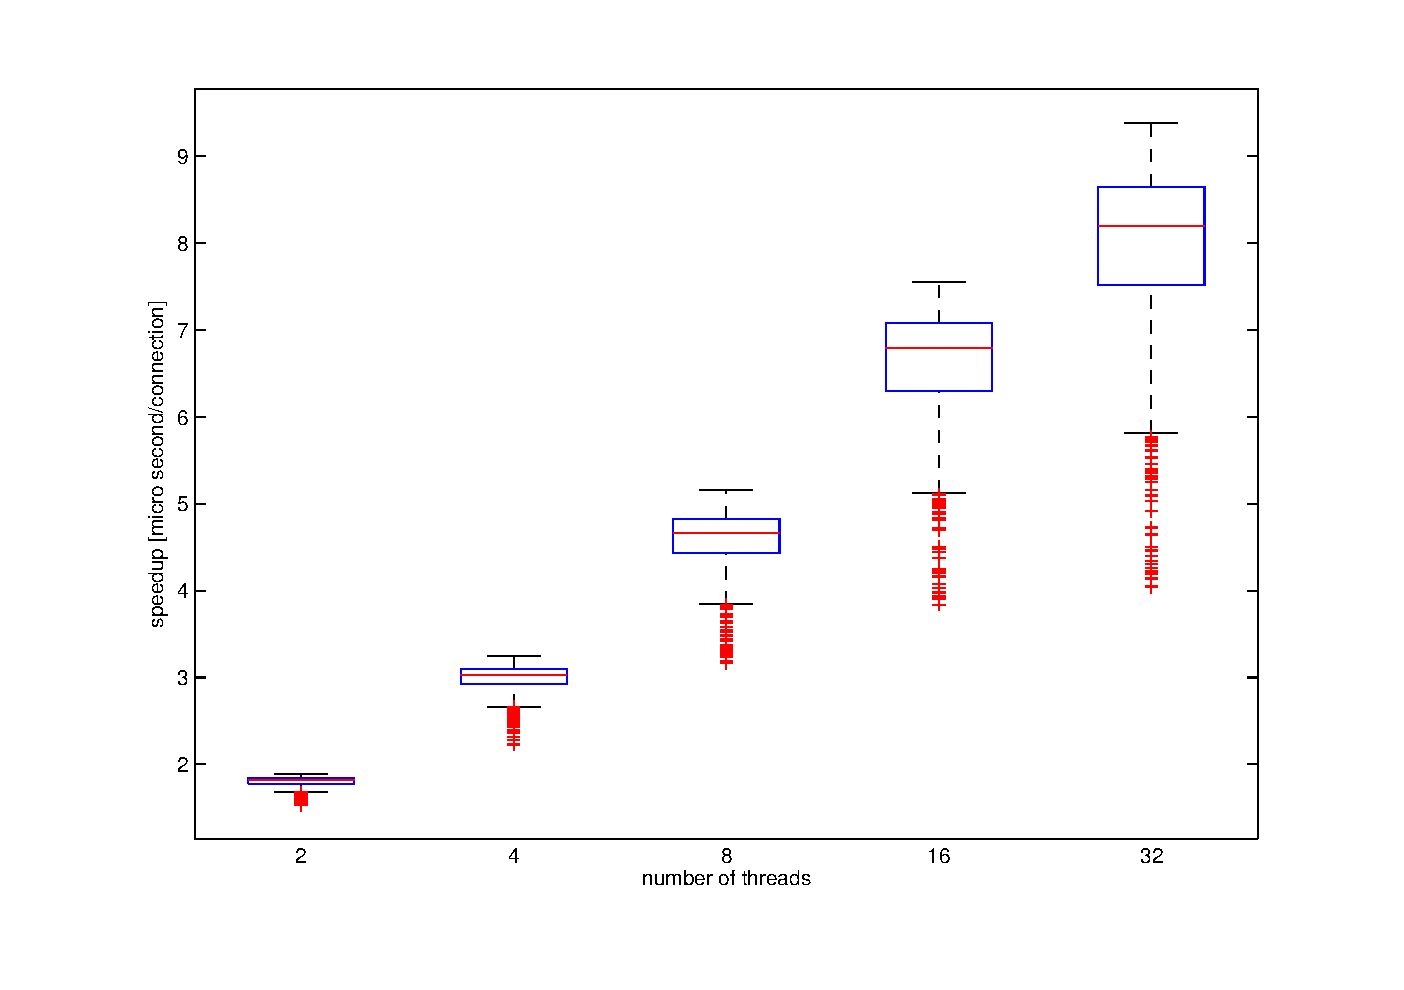
\includegraphics[scale=0.5]{pictures/boxplot_new_con_dt_1_300_speedup.eps}
\caption{The speed-up of the connection frequency per process for different number of threads is shown.
The plot shows histograms of measured values using the threehundredths circuit.}
\label{boxplotnewcon}
\end{figure}
Each thread iterates over all synapses, but only stores the connection if the post-synaptic neuron is located on
the thread. Thus the connection frequency per thread varies.
As for nodes the neurons are distributed in the modules fashion on the threads for one node.
The distribution properties are the same. Thus there is a larger variation on a larger number of threads.
Figure \ref{boxplotnewcon} shows measured connection frequencies for the connect step. The measurements are
extracted from the execution of the threehundredths circuit. It is executed on 128 nodes with varying number of
threads. The circuit plus fixed number of nodes specify the distribution of neurons per node.

A larger number of threads leads to smaller wall-clock timings, but the chance of imbalance increases.
The variations of the timings correlates with the distribution of synapses per node (figure \ref{fullcircuitdist}).
To look into detail, figure \ref{detailnewcon:second} shows the measured wall-clock time for each node
plotted over the maximum number of new connections per thread. It shows a strong correlation between the variable and
the duration. Thus the increasing variations of timings can be explained by the variations of synapses per thread.
The figure indicates two different timings per connection. There is an offset of regression between the pink
(left point cloud)
and the red (right point cloud) dots. Pink an red dots represent all measurements with less than 40,000 and more than new synapses per
node respectively. Figure \ref{detailnewcon:first} shows the density of number of new synapses per node.
Less synapses results in a smaller vector size. There seems to be a loss of efficiency, which properly result from
the use of different cache levels. 

\begin{figure}[ht!]
     \begin{center}
        \subfigure[Histogram showing measured densities of number of new synapses per iteration step for one process.]{%
            \label{detailnewcon:first}
            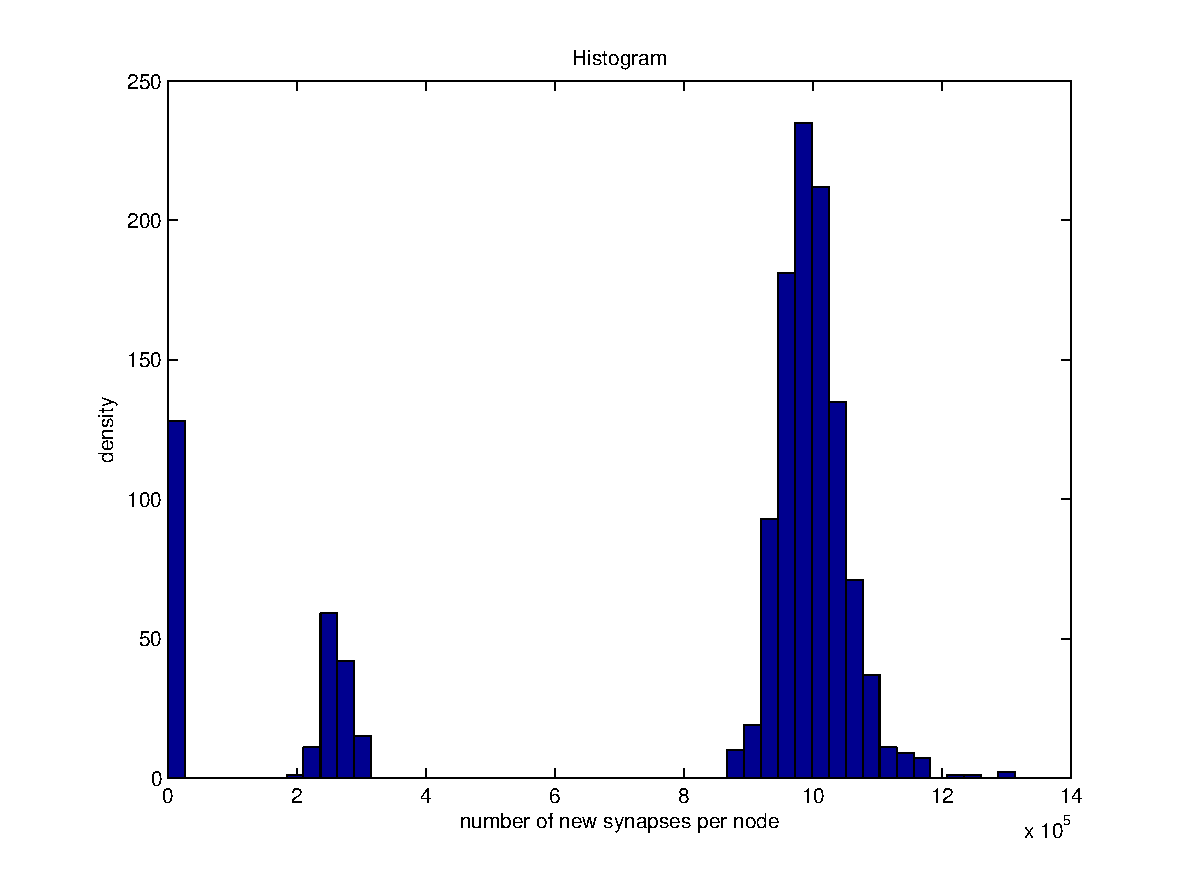
\includegraphics[scale=0.41]{pictures/histogram_new_const_1_300.eps}
        }
        \subfigure[Plotted wall-clock timings of \emph{connect} step over the number of new synapses for one thread
        			(Thread is part of process from Figure \ref{detailnewcon:first}. The new synapses are part of the new synapses from the process).
        			Pinks and red dotes relate to iterations, where the number of new synapses is smaller and bigger than $4*10^5$,
        			respectively (The values relate to the hills from Figure \ref{detailnewcon:first}). 
        			]{%
           \label{detailnewcon:second}
           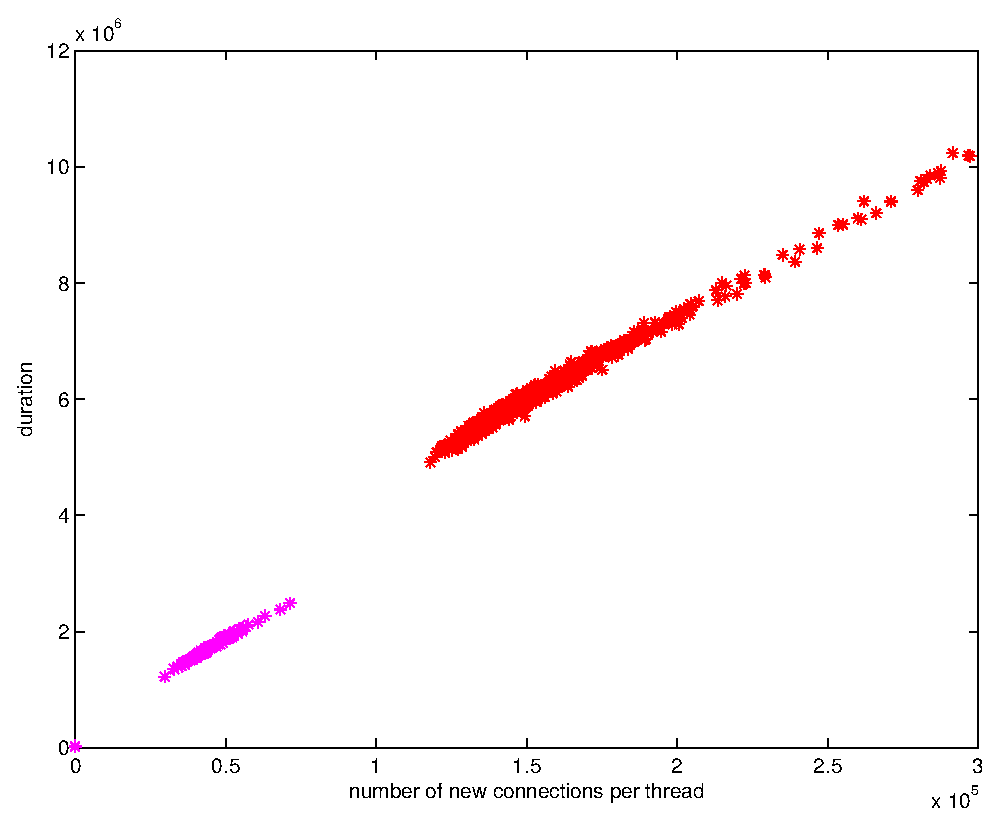
\includegraphics[scale=0.41]{pictures/t8_duration_per_con_1_300.eps}
		}
    \end{center}
    \caption{%
        The measurements are taken the same simulation run with the 1per300 circuit. It is run on the Blue Brain IV.
     }%
   \label{detailnewcon}
\end{figure}

\section{Memory consumption}
During the development of the import module, the goal to fit the full mouse brain model on the
Blue Brain IV seemed to get unrealistic. The full machine does not deliver enough memory resources.
Test runs on different scales on the JUQUEEN should give concrete results.
We extended the import module with a logging of imported synapses and the used memory.
We used a BGQ library (see Appendix \ref{bgqmemory}) to measure the current memory usage after each iteration on each process. The runs on $6$ and $8$ racks executed successfully.
The run on $4$ racks broke before. It run out of memory and crashed therefore.
\begin{figure}[h!]
\begin{center}
 \includegraphics[width=0.8\textwidth]{pgfplots/newconnections.pdf}
\end{center}
\caption{Measured new connections per node.
 }
\label{fig:newconnections}
\end{figure}
Figure \ref{fig:newconnections} shows the number of new connections per node for the different runs.
The vertical distance between the dashed and the dotted line reflects the imbalance of synapses between the nodes. Remarkable is the fact, that the imbalance is similar for the three different scales.
It enables a precise prediction of the needed memory per process.
\begin{figure}[h!]
\begin{center}
 \includegraphics[width=0.8\textwidth]{pgfplots/memory_plot.pdf}
\end{center}
\caption{Measured memory usage.
 }
\label{fig:memoryplot}
\end{figure}
Figure \ref{fig:memoryplot} shows the memory usage per node for the different runs.
The black solid line illustrates the memory limit of each node of the IBM Blue Gene /Q.
You can see that for 4 racks the full mouse brain model does not fit into memory.
Even tough an imbalance compensation would not make the model fit. 

%\subsection{Long range connection generation}



%\subsection{Short range connection generation}
%\subsection{Load circuit}

\newpage
\section{Usability for Scientists}

\subsection{Manipulation of circuit}

The connection generation implementations accept a set of command line arguments.
The arguments allow to influence the program execution.
All accepted arguments are listed in table \ref{tab:longrangeargs}.
Besides data path manipulations the voxel experiment assignment can be 
manipulated on different levels. The number of used experiments can be specified
and limited. Further, the interpolation can be enabled and limited to a range.
Also, the the available voxel information can be mirrored to the other hemisphere.
Apart from this, the voxel experiment assignment can be exported to a file.
This file can be manipulated externally and imported again.

The weights of all created synapses can be strengthened by a set factor.
This is necessary for reduces models.

The 
\begin{table}[ht!]
\begin{centering}
    \begin{tabular}{ | c | l | p{7cm} |}
    \hline
    Argument & expected type & function \\ \hline \hline
    \emph{-e} & path & set path to file, which contains picked experiment ids \\ \hline
    \emph{-n} & path & path to input neuron file \\ \hline
    \emph{-h} & path &  output folder\\ \hline
    \emph{-s} & - &  save voxel information\\ \hline
    \emph{-l} & path &  load voxel information\\ \hline
    \emph{-o} & - &  enable voxel interpolation\\ \hline
    \emph{-x} & - &  enable mirroring of voxels\\ \hline
    \emph{-c} & integer & only use one experiment with given id \\ \hline
    \emph{-m} & integer & limit number of loaded experiments \\ \hline
    \emph{-d} & integer & limit search distance for voxel interpolation \\ \hline
    \emph{-i} & integer & strengthening of weights for each synapse \\ \hline
    \end{tabular}
    \caption{Long range generation arguments to influence program execution.}
    \label{tab:longrangeargs}
\end{centering}
\end{table}

The short range generation only accepts path manipulations and weight strengthening.
The arguments are listed in table \ref{tab:shortrangeargs}.
\begin{table}[ht!]
\begin{centering}
    \begin{tabular}{ | c | l | p{7cm} |}
    \hline
    Argument & expected type & function \\ \hline \hline
    \emph{-n} & path & path to input neuron file \\ \hline
    \emph{-h} & path &  output folder\\ \hline
    \emph{-i} & integer & strengthening of weights for each synapse \\ \hline
    \end{tabular}
    \caption{Short range generation arguments to influence program execution.}
    \label{tab:shortrangeargs}
\end{centering}
\end{table}

\subsection{Import neurons}
The import neuron module can be executed with the function \emph{SLI} function  \emph{H5NeuronCsX\_s\_s\_a\_s}. It loads all neurons from the specified with its parameters
from the given HDF5 file. The function expects 4 input parameters:
\begin{itemize}
      \item Name of the a subnet dataset (String).
The subset has to contain for each neuron an integer value.
The neurons are grouped together by this subnet value.
      \item A list of all datasets which values are interpreted as list of parameters.
      \item Name of the used neuron model
      \item path to the HDF5 file 
\end{itemize}
It returns the neuron id of the first neuron it created.
\begin{lstlisting}[label=sliNeurons,caption=Calling the neuron import module via H5NeuronCsX\_s\_s\_a\_s SLI command ]
/nmodel /aeif_cond_exp def
/subnet (subnet) def
/nparameters [(C_m) (Delta_T) (E_L) (V_reset) (V_th) (a) (b)] def
/filepath (circuit/ptneu_brain.h5) def
subnet nparameters nmodel filepath H5NeuronCsX\_s\_s\_a\_s /offset Set
\end{lstlisting}

\subsection{Import synapses}
The import neuron module can be executed with the function \emph{SLI} function  \emph{H5SynapseTll\_i\_s\_a\_s}. It loads all synapses with its given parameters
from the given HDF5 file. The function expects 4 input parameters:
 
\begin{itemize}
      \item Offset of the neuron ids. Mostly it is equal to first neuron id returned by \emph{H5NeuronCsX\_s\_s\_a\_s}

      \item A list of all columns which values are interpreted as parameters.
      
      \item Name of the used synapse model
      
      \item path to the HDF5 file 
\end{itemize}

\begin{lstlisting}[label=sliSynapses,caption=Example importing synapses]
/synmodel /tsodyks2_synapse def
/synparams [(delay) (weight) (U0) (TauRec) (TauFac)] def
/filepath (circuit/syn.h5) def
offset synparams synmodel filepath H5SynapseTll_i_s_a_s
\end{lstlisting}

\subsection{NEST simulation options}

Only one use-case (\ref{ambmusecase}) of the mouse brain model is used in this thesis for performance evaluations.
Never the less more use-cases are realizable with the given implementations.
In general the neuron load module can be used equivalent to the neuron create function
and the synapses load module can be used equivalent to the neuron connect function.
Further, a given circuit can be loaded and adapted (use offset or scaling factor for parameters).
Loaded neurons can be divided into subsets. The \emph{SLI} functionality allows to access neuron sets
from subnets. Thus the grouping performed with the subnet dataset is available for all \emph{SLI} functions.
Stimulus generator and \emph{Spikedetector} or \emph{Multimeter} can be used to stimulate
and observe specific neurons, respectively.
More use-cases are possible: For example the \emph{SLI} connect functions can be used to strengthening or weakening the connections between two
parts of the circuit.

\subsection{Conclusion}
The implementations presented in chapter 2 allow to run a data-driven simulation using the neuronal simulator NEST.
A pipeline for generating connections from different sources is implemented, which can handle the amount of data needed for 
a full mouse brain simulation. Further, presented visualisation tools allow to analyse the neuronal activity.
Besides a demonstration of today's possibilities, the work in this thesis extends the neuronal simulator with the feature of loading well-defined
point neuron circuits. An integration of the new import functionality into the \emph{SLI}
interface allows to extend current simulations with well-defined circuit data easily.
As more data is available data-driven neuronal simulations will gain further importance.

The used data format is not optimized for the NEST data structure. It stores the circuit data in general way 
to not put any obstacles in the way to use the proposed data format for different use-cases.

The achieved performance of importing the circuit is feasible. Anyway improvements are possible.
For example, a multi core sort algorithm could speed-up the sort set.
Additionally gain could be gotten by optimizing the core of NEST for the build-up procedures.

\section{Prospect}
The introduced pipeline to run large scale data-driven simulation is still experimental.
Even tough, validations are introduced and manipulation functionalities are included, the 
implementations are only used and tested for the given use-case. Further, building a given 
mouse brain model directs the proposed efficiency requirements. Taking into account that
the mouse brain model is still in development, more efficient implementations of the 
circuit generation could be of need. Scalability runs of the circuit generation could
highlight bottlenecks. Additionally more general unit test should be introduced.

The NEST import modules are only accessible via the SLI interface.
To make it usable for more users the import modules should be integrated into the Python
interface as well. Further, the generated circuit is distributed uniformly by NEST on the processes. But this is not guaranteed. Therefore it might me necessary to include reshuffling of neuron distribution to achieve better memory and load balancing in the pipeline.

The simulated mouse brain model does not produce expected activity yet.
The introduced validation are only taking the correct implementation of the algorithms into account.
But the given model was never created and simulation on the full scale. Therefore the expected outcome is unclear. As soon as the model produces more sense full results, visualisation techniques from the
Blue Brain Project and the RWTH Aachen can gives insight of the model behaviour.

